\chapter{Introduction to Systems of Systems and Game Theory}
% \assignment{ 
\begin{itemize}
\item Z. Han, D. Niyato, W. Saad, T. Basar, A. Hjørungnes. Game Theory in Wireless and Communication Networks:
  Theory, Models, and Applications. Cambridge University Press 2012. Chapters 3.1, 3.2
\item A. MacKenzie, L. DaSilva. Game Theoryfor Wireless Engineers. Morgan \& Claypool Publishers. 2006. Chapter
  3.
\end{itemize} 
% }

\assignment{
  \textbf{Problem 1 - Prisoners Dilemma} \\
  Two suspects are arrested for a crime and placed in two isolated rooms. Each ones of the suspects has 
  to decide whether or not to confess and implicate the other. The rules are the following. If none of the 
  suspects confesses, then each will serve 2 years in jail. If both of them confess and implicate each other, 
  they will both go to prison for 4 years. However, if one prisoner confesses and implicates the other while 
  the other one does not confess, the one who has cooperated with the police will be set free, while the 
  other will spend 5 years in prison.\\
  % Define who players in this game are and what the possible strategies are. Formulate the game in 
  % strategic form (give a matrix representation of the game). Is this game a zero‐sum game or not‐zero‐
  % sum game? Are there any dominating strategies? Find Nash equilibrium.
  \begin{enumerate}
  \item Define who are the players
  \item What are the possible strategies
  \item Formulate in matrix representation.
  \item Is the game zero-sum game?
  \item Are there any dominating strategies?
  \item Find Nash the equilibrium.
  \end{enumerate}
}
\section{Problem 1 - Solution}
\begin{enumerate}
\item \textbf{Define who are the players:} There are two players in the game - The two prisoners
\item \textbf{What are the possible strategies:} The strategy space $S = (0,1)$ \\
  where 0 is not to confess and implicate the other                             \\
  and 1 is to confess.
\item \textbf{Formulate in matrix representation:} The matrix representation
  \begin{center}
    \begin{tabular}{ r|c|c| }
      \multicolumn{1}{r}{}
      & \multicolumn{1}{c}{$s_2 = 0$}
      & \multicolumn{1}{c}{$s_2 = 1$}                                   \\
      \cline{2-3}
      $s_1 = 0$ & $(2,2)$ & $(5,0)$                                               \\
      \cline{2-3}
      $s_1 = 1$ & $(0,5)$ & $(4,4)$                                               \\
      \cline{2-3}
    \end{tabular}
  \end{center}
\item \textbf{Is the game zero-sum game:}
\item \textbf{Are there any dominating strategies:} The dominating strategies is to confess $s_i = 1$
\item \textbf{Find Nash the equilibrium:} The Nash equilibrium is $(4,4)$, this is because of the fact that none of the
  players can gain from changing strategy at this point taking the other players choice in consideration. If whichever of
  the prisoners changes strategy from this point it will cause a less favorable outcome for the prisoner in question.

  There is a global minimum at (2,2), but this is an unstable minimum where both of the prisoners can gain, from
  changing strategy.
\end{enumerate}

\assignment{
  \textbf{Problem 2 - Multipath Routing} \\
  Imagine that there 4 nodes A, B, C and D linked as it is shown on the figure. User 1 would like to send his 
  data packets from B to D; user 2 would like to send his packets from A to C. First user can chose a route 
  B-A-D or B-C-D. There are also two choices for the second user: A-B-C and A-D-C. Throughput 
  experienced by a user depends on whether he is using a link alone or it is shared with another user. The 
  vectors (a; b) attached to each link denotes a throughput a user experiencing over the link: a if he is 
  doing it alone alone, and b if he shares it with another user.\\
  % Write a matrix to describe this game. Investigate if the game has Nash equilibrium and what would be a 
  % rational choice for the two users.  
  \begin{enumerate}
  \item Formulate in matrix representation.
  \item Find Nash equilibrium.
  \item What would be the rational choice?
  \end{enumerate}

  \begin{figure}[H]
    \centering
    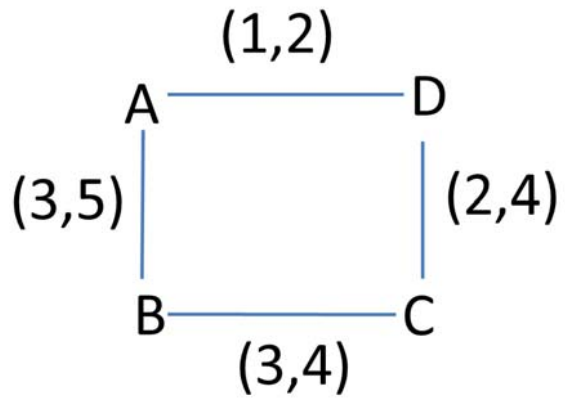
\includegraphics[width=0.35\textwidth]{gt_network_ex2.png}
  \end{figure}
}

\section{Problem 2 - Solution}
\begin{enumerate}
\item The matrix representation \\
  \begin{tabular}{ r|c|c| }
    \multicolumn{1}{r}{}
    &  \multicolumn{1}{c}{$s_2 = A-B-C$}
    & \multicolumn{1}{c}{$s_2 = A-D-C$} \\
    \cline{2-3}
    $s_1 = B-A-D$ & $(6,8)$ & $(5,4)$ \\
    \cline{2-3}
    $s_1 = B-C-D$ & $(6,7)$ & $(7,5)$ \\
    \cline{2-3}
  \end{tabular}
\item The Nash equilibrium is $(5,4)$ where player 1 choose $B-A-D$ and player 2 choose $A-D-C$
\end{enumerate}
